% Migrata dal Cap. 5 per il vincolo di lunghezza del corpo.
% Nel capitolo resta il paragrafo di raccordo con i tre fatti usati nel seguito.

\subsection{L'Anatomia Fisica di una QPU}

Per capire dove nascono gli errori bisogna prima capire com'è fatta la macchina. Una \ac{QPU} superconduttiva è un chip criogenico che contiene \emph{esclusivamente} i qubit e le linee fisiche che li collegano: contrariamente all'intuizione, \textbf{le porte logiche non risiedono nel chip}. Aprendo una CPU classica si trovano registri e porte logiche incise nel silicio; aprendo una QPU si trovano solo i qubit. Le operazioni sono realizzate dall'\textbf{elettronica di controllo esterna}, che invia impulsi a microonde convogliati ai qubit tramite guide d'onda: ``far passare un qubit in un gate'' significa in realtà inviargli un'onda sagomata che ne ruota lo spin dell'angolo desiderato (90°, 30°, 10°, \ldots). La Figura~\ref{fig:qpu_anatomia} schematizza questa architettura per una QPU a 5 qubit con topologia a catena lineare.

\begin{figure}[H]
\centering
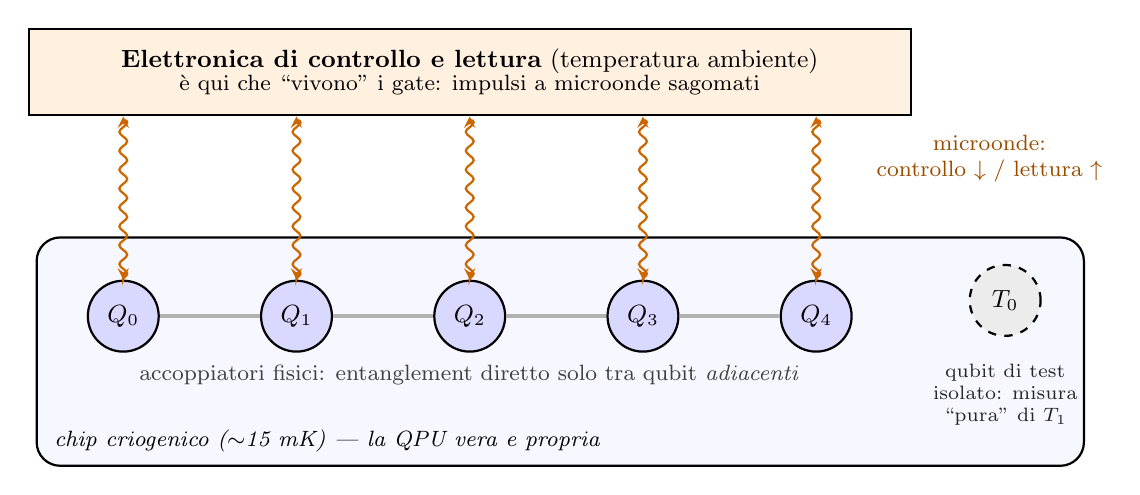
\begin{tikzpicture}[
  qubit/.style={circle, draw=black, thick, fill=blue!15, minimum size=9mm, font=\small},
  testq/.style={circle, draw=black, thick, dashed, fill=gray!15, minimum size=9mm, font=\small},
  wave/.style={decorate, decoration={snake, amplitude=0.5mm, segment length=2.4mm}, thick, <->, >=stealth, orange!80!black},
  coupl/.style={line width=1.6pt, gray!60}
]
% elettronica di controllo
\node[rectangle, draw=black, thick, fill=orange!12, minimum width=112mm, minimum height=11mm, align=center, font=\small] (E) at (4.4, 3.1)
  {\textbf{Elettronica di controllo e lettura} (temperatura ambiente)\\[-1mm] {\footnotesize è qui che ``vivono'' i gate: impulsi a microonde sagomati}};
% chip
\draw[rounded corners=3mm, thick, fill=blue!3] (-1.1,-1.9) rectangle (12.2,1.0);
\node[font=\footnotesize\itshape, anchor=south west] at (-1.0,-1.85) {chip criogenico ($\sim$15 mK) --- la QPU vera e propria};
% qubit di calcolo
\node[qubit] (Q0) at (0,0) {$Q_0$};
\node[qubit] (Q1) at (2.2,0) {$Q_1$};
\node[qubit] (Q2) at (4.4,0) {$Q_2$};
\node[qubit] (Q3) at (6.6,0) {$Q_3$};
\node[qubit] (Q4) at (8.8,0) {$Q_4$};
% accoppiatori
\draw[coupl] (Q0) -- (Q1);
\draw[coupl] (Q1) -- (Q2);
\draw[coupl] (Q2) -- (Q3);
\draw[coupl] (Q3) -- (Q4);
\node[font=\footnotesize, gray!50!black] at (4.4,-0.75) {accoppiatori fisici: entanglement diretto solo tra qubit \emph{adiacenti}};
% qubit di test isolati
\node[testq] (T0) at (11.2,0.2) {$T_0$};
\node[font=\scriptsize, align=center, gray!30!black] at (11.2,-1.0) {qubit di test\\isolato: misura\\``pura'' di $T_1$};
% onde
\foreach \q in {Q0,Q1,Q2,Q3,Q4}{ \draw[wave] (E.south -| \q) -- (\q.north); }
\node[font=\footnotesize, orange!60!black, align=center] at (11.0,2.0) {microonde:\\controllo $\downarrow$ / lettura $\uparrow$};
\end{tikzpicture}
\caption[Anatomia di una QPU superconduttiva a 5 qubit (topologia a catena)]{Anatomia di una \ac{QPU} superconduttiva a 5 qubit con topologia a catena lineare. Nel chip criogenico risiedono solo i qubit e gli accoppiatori fisici; le porte logiche sono impulsi a microonde generati dall'elettronica esterna e convogliati tramite guide d'onda, usate sia per il controllo sia per la lettura. L'entanglement diretto è possibile solo tra qubit adiacenti ($Q_1$--$Q_2$ sì, $Q_0$--$Q_2$ solo tramite operazioni intermedie, che amplificano il disturbo). Il qubit di test $T_0$, privo di collegamenti, serve a misurare il tempo di coerenza ``puro'': un qubit collegato a una guida d'onda perde sempre un po' di energia attraverso di essa.}
\label{fig:qpu_anatomia}
\end{figure}

La Figura~\ref{fig:qpu_reale} mostra come questa architettura si presenta nella realtà: all'esterno il sistema integrato (criostato, elettronica e schermature racchiusi nella teca), all'interno della sala macchine i cilindri criogenici sospesi con il fascio di tubi e cavi coassiali che convogliano le microonde di controllo e lettura --- le ``guide d'onda'' dello schema precedente.

\begin{figure}[H]
\centering
\subfloat[IBM Quantum System One (Ehningen, Germania)]{
\includegraphics[height=52mm]{foto_system_one.jpg}}\hspace{3mm}
\subfloat[Criostati IBM Q con il cablaggio di controllo]{
\includegraphics[height=52mm]{foto_criostato_ibm.jpg}}
\caption[La QPU reale: sistema integrato e criostati con cablaggio]{La \ac{QPU} reale. (a)~Il sistema integrato IBM Quantum System One: il cilindro nero al centro è il criostato che contiene il chip, circondato dall'elettronica di controllo. (b)~Criostati IBM Q in sala macchine: dall'alto arrivano i tubi per la refrigerazione e i cavi coassiali che convogliano le microonde di controllo e lettura verso il chip, sospeso sul fondo del cilindro a $\sim$15\,mK. \emph{Crediti: (a) IBM Research, licenza CC~BY~2.0; (b) Connie Zhou per IBM, pubblico dominio; entrambe via Wikimedia Commons.}}
\label{fig:qpu_reale}
\end{figure}

\begin{figure}[H]
\centering

\includegraphics[width=0.62\textwidth]{foto_chip_transmon.png}
\caption[Chip quantistico superconduttivo a 6 transmon con giunzioni di test]{Resa tridimensionale di un chip quantistico superconduttivo con 6 qubit transmon e 12 giunzioni di test. Si riconoscono gli elementi dello schema di Figura~\ref{fig:qpu_anatomia}: i qubit con i loro risonatori, le linee di accoppiamento, le piazzole dorate per il collegamento alle guide d'onda e --- ai quattro angoli --- le strutture di test isolate, l'analogo reale del qubit $T_0$. \emph{Credito: Onri Jay Benally, licenza CC~BY~4.0, via Wikimedia Commons.}}
\label{fig:chip_transmon}
\end{figure}

Questa architettura ha tre conseguenze dirette per gli errori.

\paragraph{La lettura distrugge lo stato --- fisicamente.}
Anche la misura avviene tramite microonde: per leggere un qubit lo si ``bombarda'' con un'onda di sonda e si osserva come essa torna indietro --- un modo di risposta corrisponde a $\ket{0}$, un altro a $\ket{1}$. L'atto stesso di sondare blocca la dinamica del qubit: è per questo che la misura di uno stato quantistico lo distrugge \emph{realmente}, non per convenzione matematica. Ed è per questo che nei circuiti le letture stanno tutte alla fine, in parallelo: misurare un solo qubit lasciando gli altri in sovrapposizione significa inviare un'onda che, per quanto focalizzata, perturba anche i vicini e può farli precipitare.

\paragraph{Il budget di operazioni: coerenza vs velocità dei gate.}
Le prestazioni di una QPU dipendono dal rapporto tra due tempi: quanto a lungo il qubit resta coerente e quanto dura una singola operazione. Con una finestra di coerenza di $100\,\mu$s e gate da $\sim$25\,ns, si eseguono $\sim$4\,000 operazioni; una macchina con coerenza superiore ma gate più lenti può eseguirne \emph{meno}. È il rapporto che conta, non il singolo parametro --- ed è questo rapporto a decidere se il circuito di Shor per una data istanza è fisicamente eseguibile. La Tabella~\ref{tab:tecnologie_qpu} confronta gli ordini di grandezza delle due principali tecnologie.

\begin{table}[H]
\centering
\resizebox{\textwidth}{!}{%
\begin{tabular}{@{}lll@{}}
\toprule
 & \textbf{Superconduttori (IBM, IQM, \ldots)} & \textbf{Ioni intrappolati (IonQ, Quantinuum, \ldots)} \\
\midrule
Tempo di coerenza          & $50$--$300\,\mu$s                      & da secondi a minuti \\
Durata gate (1 qubit)      & $\sim$15--40\,ns                       & $\sim$1--100\,$\mu$s \\
Durata gate (2 qubit)      & $\sim$60--500\,ns                      & $\sim$0.1--1\,ms \\
Operazioni per finestra    & $\sim 10^{3}$--$10^{4}$                & $\sim 10^{3}$ \\
Lettura                    & più esposta a errori e interferenze     & più stabile e affidabile \\
Crosstalk                  & presente (accoppiamento capacitivo)     & ridotto \\
Velocità di esecuzione     & molto alta                              & bassa (gate lenti) \\
\bottomrule
\end{tabular}%
}
\caption[Confronto tra tecnologie di QPU: superconduttori vs ioni intrappolati]{Ordini di grandezza indicativi delle due principali tecnologie di \ac{QPU}. La coerenza lunghissima degli ioni intrappolati non si traduce in più operazioni utili, perché i gate sono da $10^3$ a $10^4$ volte più lenti: il budget di operazioni per finestra di coerenza è simile, ma i superconduttori lo spendono molto più in fretta. Gli ioni sono invece più robusti su lettura e crosstalk.}
\label{tab:tecnologie_qpu}
\end{table}

\paragraph{Il bordo di coerenza.}
Gli errori non sono distribuiti uniformemente nel tempo: finché il calcolo occupa una piccola frazione della finestra di coerenza, la probabilità di decadimento è bassa; quando il circuito si spinge \emph{verso la fine} della finestra --- il ``bordo di coerenza'' --- la probabilità che il qubit sia già decaduto al momento della misura cresce rapidamente. La Figura~\ref{fig:bordo_coerenza} illustra il concetto: è la ragione per cui circuiti profondi come quello di Shor, che consumano gran parte del budget, producono letture inaffidabili anche quando ``tecnicamente'' rientrano nella finestra.

\begin{figure}[H]
\centering
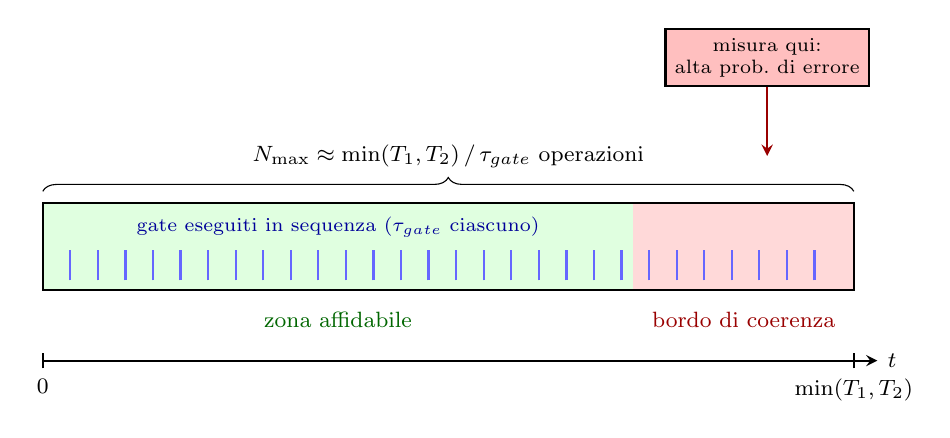
\begin{tikzpicture}[>=stealth]
% finestre
\fill[green!12] (0,0) rectangle (7.5,1.1);
\fill[red!15]   (7.5,0) rectangle (10.3,1.1);
\draw[thick] (0,0) rectangle (10.3,1.1);
% gate ticks
\foreach \x in {0.35,0.7,...,9.8}{ \draw[blue!60, thick] (\x,0.12) -- (\x,0.5); }
\node[font=\scriptsize, blue!60!black, fill=green!12, inner sep=1.5pt] at (3.75,0.8) {gate eseguiti in sequenza ($\tau_{\text{gate}}$ ciascuno)};
% etichette zone
\node[font=\footnotesize, green!40!black] at (3.75,-0.38) {zona affidabile};
\node[font=\footnotesize, red!60!black]   at (8.9,-0.38) {bordo di coerenza};
% asse tempo
\draw[->, thick] (0,-0.9) -- (10.6,-0.9) node[right, font=\footnotesize] {$t$};
\draw[thick] (0,-1.0) -- (0,-0.8) node[below=2mm, font=\footnotesize] {$0$};
\draw[thick] (10.3,-1.0) -- (10.3,-0.8) node[below=2mm, font=\footnotesize] {$\min(T_1, T_2)$};
% graffa budget
\draw[decorate, decoration={brace, amplitude=5pt}] (0,1.25) -- (10.3,1.25)
  node[midway, above=5pt, font=\footnotesize] {$N_{\max} \approx \min(T_1,T_2)\,/\,\tau_{\text{gate}}$ operazioni};
% misura
\node[draw, thick, fill=red!25, font=\scriptsize, align=center] (M) at (9.2,2.95) {misura qui:\\alta prob.\ di errore};
\draw[->, thick, red!60!black] (M.south) -- (9.2,1.7);
\end{tikzpicture}
\caption[Il bordo di coerenza: budget di operazioni e rischio di misura]{Il ``budget'' di operazioni di un qubit: la finestra di coerenza $\min(T_1, T_2)$ divisa per la durata del singolo gate dà il numero massimo di operazioni eseguibili $N_{\max}$. Un circuito che consuma solo la prima parte della finestra opera in zona affidabile; un circuito profondo come quello di Shor spinge la misura verso il \emph{bordo di coerenza}, dove la probabilità che il qubit sia già decaduto --- e che la lettura restituisca un valore errato --- è massima.}
\label{fig:bordo_coerenza}
\end{figure}

\paragraph{La topologia decide chi parla con chi.}
Le QPU differiscono anche per geometria: catene lineari, griglie (heavy-hex di IBM), connettività completa. Su una catena, l'entanglement tra qubit non adiacenti richiede un ``cross-entanglement'' attraverso i qubit intermedi: ogni passaggio disperde energia e accorcia la vita dello stato condiviso --- più cross si fanno, prima lo stato decade. La topologia determina quindi sia \emph{quali} circuiti si possono mappare in modo efficiente, sia \emph{dove} il crosstalk colpirà. Questo aspetto --- insieme al fatto che i parametri di coerenza variano da qubit a qubit dello stesso chip --- è ripreso nel Capitolo~\ref{chap:surface}, dove la località delle interazioni sulla griglia è il fondamento architetturale del surface code.
